\documentclass[]{book}
\usepackage{lmodern}
\usepackage{amssymb,amsmath}
\usepackage{ifxetex,ifluatex}
\usepackage{fixltx2e} % provides \textsubscript
\ifnum 0\ifxetex 1\fi\ifluatex 1\fi=0 % if pdftex
  \usepackage[T1]{fontenc}
  \usepackage[utf8]{inputenc}
\else % if luatex or xelatex
  \ifxetex
    \usepackage{mathspec}
  \else
    \usepackage{fontspec}
  \fi
  \defaultfontfeatures{Ligatures=TeX,Scale=MatchLowercase}
\fi
% use upquote if available, for straight quotes in verbatim environments
\IfFileExists{upquote.sty}{\usepackage{upquote}}{}
% use microtype if available
\IfFileExists{microtype.sty}{%
\usepackage{microtype}
\UseMicrotypeSet[protrusion]{basicmath} % disable protrusion for tt fonts
}{}
\usepackage[unicode=true]{hyperref}
\PassOptionsToPackage{usenames,dvipsnames}{color} % color is loaded by hyperref
\hypersetup{
            pdftitle={Saemix: Open Source R package for mixed effects modeling},
            pdfauthor={Marc Lavielle, Emmanuelle Comets, Audrey Lavenu and Belhal Karimi},
            colorlinks=true,
            linkcolor=Maroon,
            citecolor=Blue,
            urlcolor=blue,
            breaklinks=true}
\urlstyle{same}  % don't use monospace font for urls
\usepackage{natbib}
\bibliographystyle{apalike}
\usepackage{color}
\usepackage{fancyvrb}
\newcommand{\VerbBar}{|}
\newcommand{\VERB}{\Verb[commandchars=\\\{\}]}
\DefineVerbatimEnvironment{Highlighting}{Verbatim}{commandchars=\\\{\}}
% Add ',fontsize=\small' for more characters per line
\usepackage{framed}
\definecolor{shadecolor}{RGB}{248,248,248}
\newenvironment{Shaded}{\begin{snugshade}}{\end{snugshade}}
\newcommand{\KeywordTok}[1]{\textcolor[rgb]{0.13,0.29,0.53}{\textbf{{#1}}}}
\newcommand{\DataTypeTok}[1]{\textcolor[rgb]{0.13,0.29,0.53}{{#1}}}
\newcommand{\DecValTok}[1]{\textcolor[rgb]{0.00,0.00,0.81}{{#1}}}
\newcommand{\BaseNTok}[1]{\textcolor[rgb]{0.00,0.00,0.81}{{#1}}}
\newcommand{\FloatTok}[1]{\textcolor[rgb]{0.00,0.00,0.81}{{#1}}}
\newcommand{\ConstantTok}[1]{\textcolor[rgb]{0.00,0.00,0.00}{{#1}}}
\newcommand{\CharTok}[1]{\textcolor[rgb]{0.31,0.60,0.02}{{#1}}}
\newcommand{\SpecialCharTok}[1]{\textcolor[rgb]{0.00,0.00,0.00}{{#1}}}
\newcommand{\StringTok}[1]{\textcolor[rgb]{0.31,0.60,0.02}{{#1}}}
\newcommand{\VerbatimStringTok}[1]{\textcolor[rgb]{0.31,0.60,0.02}{{#1}}}
\newcommand{\SpecialStringTok}[1]{\textcolor[rgb]{0.31,0.60,0.02}{{#1}}}
\newcommand{\ImportTok}[1]{{#1}}
\newcommand{\CommentTok}[1]{\textcolor[rgb]{0.56,0.35,0.01}{\textit{{#1}}}}
\newcommand{\DocumentationTok}[1]{\textcolor[rgb]{0.56,0.35,0.01}{\textbf{\textit{{#1}}}}}
\newcommand{\AnnotationTok}[1]{\textcolor[rgb]{0.56,0.35,0.01}{\textbf{\textit{{#1}}}}}
\newcommand{\CommentVarTok}[1]{\textcolor[rgb]{0.56,0.35,0.01}{\textbf{\textit{{#1}}}}}
\newcommand{\OtherTok}[1]{\textcolor[rgb]{0.56,0.35,0.01}{{#1}}}
\newcommand{\FunctionTok}[1]{\textcolor[rgb]{0.00,0.00,0.00}{{#1}}}
\newcommand{\VariableTok}[1]{\textcolor[rgb]{0.00,0.00,0.00}{{#1}}}
\newcommand{\ControlFlowTok}[1]{\textcolor[rgb]{0.13,0.29,0.53}{\textbf{{#1}}}}
\newcommand{\OperatorTok}[1]{\textcolor[rgb]{0.81,0.36,0.00}{\textbf{{#1}}}}
\newcommand{\BuiltInTok}[1]{{#1}}
\newcommand{\ExtensionTok}[1]{{#1}}
\newcommand{\PreprocessorTok}[1]{\textcolor[rgb]{0.56,0.35,0.01}{\textit{{#1}}}}
\newcommand{\AttributeTok}[1]{\textcolor[rgb]{0.77,0.63,0.00}{{#1}}}
\newcommand{\RegionMarkerTok}[1]{{#1}}
\newcommand{\InformationTok}[1]{\textcolor[rgb]{0.56,0.35,0.01}{\textbf{\textit{{#1}}}}}
\newcommand{\WarningTok}[1]{\textcolor[rgb]{0.56,0.35,0.01}{\textbf{\textit{{#1}}}}}
\newcommand{\AlertTok}[1]{\textcolor[rgb]{0.94,0.16,0.16}{{#1}}}
\newcommand{\ErrorTok}[1]{\textcolor[rgb]{0.64,0.00,0.00}{\textbf{{#1}}}}
\newcommand{\NormalTok}[1]{{#1}}
\usepackage{longtable,booktabs}
\usepackage{graphicx,grffile}
\makeatletter
\def\maxwidth{\ifdim\Gin@nat@width>\linewidth\linewidth\else\Gin@nat@width\fi}
\def\maxheight{\ifdim\Gin@nat@height>\textheight\textheight\else\Gin@nat@height\fi}
\makeatother
% Scale images if necessary, so that they will not overflow the page
% margins by default, and it is still possible to overwrite the defaults
% using explicit options in \includegraphics[width, height, ...]{}
\setkeys{Gin}{width=\maxwidth,height=\maxheight,keepaspectratio}
\IfFileExists{parskip.sty}{%
\usepackage{parskip}
}{% else
\setlength{\parindent}{0pt}
\setlength{\parskip}{6pt plus 2pt minus 1pt}
}
\setlength{\emergencystretch}{3em}  % prevent overfull lines
\providecommand{\tightlist}{%
  \setlength{\itemsep}{0pt}\setlength{\parskip}{0pt}}
\setcounter{secnumdepth}{5}
% Redefines (sub)paragraphs to behave more like sections
\ifx\paragraph\undefined\else
\let\oldparagraph\paragraph
\renewcommand{\paragraph}[1]{\oldparagraph{#1}\mbox{}}
\fi
\ifx\subparagraph\undefined\else
\let\oldsubparagraph\subparagraph
\renewcommand{\subparagraph}[1]{\oldsubparagraph{#1}\mbox{}}
\fi
\usepackage{booktabs}
\usepackage{amsthm}
\makeatletter
\def\thm@space@setup{%
  \thm@preskip=8pt plus 2pt minus 4pt
  \thm@postskip=\thm@preskip
}
\makeatother

\title{\texttt{Saemix}: Open Source R package for mixed effects modeling}
\author{Marc Lavielle, Emmanuelle Comets, Audrey Lavenu and Belhal Karimi}
\date{2020-02-05}

\begin{document}
\maketitle

{
\hypersetup{linkcolor=black}
\setcounter{tocdepth}{1}
\tableofcontents
}
\chapter*{Welcome to mixed effects modeling in
R}\label{welcome-to-mixed-effects-modeling-in-r}
\addcontentsline{toc}{chapter}{Welcome to mixed effects modeling in R}

The saemix project is an R package \citep{saemix2017} available in CRAN
that implements the Stochastic Approximation of the EM (SAEM) algorithm
introduced in \citep{kuhn}. This algorithm is state-of-the-art method
for fitting, possibly non linear, models in agronomy, animal breeding or
Pharmacokinetics-Pharmacodynamics (PKPD) analysis.

Thus far, the main area using the package thus far is Pharmacology,
especially to understand how drugs, under development, behave in the
body or how the body reacts to a drug during clinical trials but we
ought to aim at a more general audience of biostatisticians dealing with
nonlinear mixed effects modeling.

\begin{figure}

{\centering 
\includegraphics[width=0.6\linewidth]{figures/logo1} 

}

\end{figure}

\texttt{saemix} is licensed under
\href{https://cran.r-project.org/web/licenses/GPL-2}{GPL-2} \textbar{}
\href{https://cran.r-project.org/web/licenses/GPL-3}{GPL-3} {[}expanded
from: GPL (\textgreater{}=2){]}.

\chapter{Introduction}\label{intro}

Longitudinal data arise in many fields, such as agronomy, spatial
analysis, imagery, clinical trials, and have been particularly prominent
in the field of pharmacokinetics (PK) and pharmacodynamics (PD), where
increasingly complex models involving mechanistic and empirical
processes have been developed to describe the time course of and
responses to drugs. Nonlinear models pose unique challenges in terms of
estimation methods, and have driven the research to provide better
estimation of parameters as well as the associated uncertainty,
diagnostics of model misspecification and more informative designs. The
SAEM algorithm, based on two highly cited publications by one of our
project members Marc Lavielle, see \citep{lavielle} and \citep{kuhn},
was implemented in R in 2011 in the \texttt{saemix} R
package\textasciitilde{}\citep{saemix2017}. Several applications of SAEM
in agronomy, animal breeding and PKPD analysis have been published using
\texttt{saemix}.

PK/PD analyses are now a fundamental element of the registration file
submitted to health authority for the approval of new drugs, but NLMEM
are also increasingly applied to other areas. In clinical trials, they
complement the point analyses by offering a unique understanding of the
evolution of disease or treatment action. In cohort studies, they allow
to model trajectories such as growth or cognitive decline. Joint models
are now routinely used to link the evolution of markers with the
occurrence of an event. Making use of S4 classes and methods to provide
user-friendly interaction, \texttt{saemix} provides a new maximum
likelihood estimation tool with a powerful exact algorithm to the R
community.

\chapter{Installation}\label{install}

\texttt{saemix} can be installed and used on several platforms.
Installation can range from easy to challenging, depending on the
platform. We are in the process of streamlining this process, and any
help or suggestions are greatly appreciated!

\section{\texorpdfstring{\texttt{CRAN}}{CRAN}}\label{cran}

You can either install the package directly from your R console

\begin{verbatim}
install.packages("saemix")
\end{verbatim}

\section{\texorpdfstring{\texttt{Github}: Build from
source}{Github: Build from source}}\label{github-build-from-source}

You can also build it from Github using the R package ``devtools''

\begin{verbatim}
library("devtools")

install_github("saemixdevelopment/saemix" )

library(saemix)
\end{verbatim}

\chapter{Materials}\label{materials}

\section{User's Guide}\label{users-guide}

\begin{itemize}
\tightlist
\item
  Saemix User's Guide: PDF
\end{itemize}

\section{Posters and Presentations}\label{posters-and-presentations}

\begin{itemize}
\tightlist
\item
  PAGE 2011, Athens, Greece: PosterPAGE
\end{itemize}

Various other publications can be found
\href{https://github.com/saemixdevelopment/Publications}{here}.

\chapter{Case Studies}\label{casestudies}

Some basic Case Studies are demonstrated in this chapter; the vignettes
will be discussing the application in more depth.

\section{A two-compartment PK model}\label{a-two-compartment-pk-model}

\begin{Shaded}
\begin{Highlighting}[]
\KeywordTok{library}\NormalTok{(saemix)}
\NormalTok{?saemix}
\end{Highlighting}
\end{Shaded}

\textbf{Read the Data}

\begin{Shaded}
\begin{Highlighting}[]
\NormalTok{warfa_data <-}\StringTok{ }\KeywordTok{read.table}\NormalTok{(}\StringTok{"data/warfarin_data.txt"}\NormalTok{, }\DataTypeTok{header=}\NormalTok{T)}
\NormalTok{saemix.data<-}\KeywordTok{saemixData}\NormalTok{(}\DataTypeTok{name.data=}\NormalTok{warfa_data,}\DataTypeTok{header=}\OtherTok{TRUE}\NormalTok{,}\DataTypeTok{sep=}\StringTok{" "}\NormalTok{,}
  \DataTypeTok{na=}\OtherTok{NA}\NormalTok{, }\DataTypeTok{name.group=}\KeywordTok{c}\NormalTok{(}\StringTok{"id"}\NormalTok{),}\DataTypeTok{name.predictors=}\KeywordTok{c}\NormalTok{(}\StringTok{"amount"}\NormalTok{,}\StringTok{"time"}\NormalTok{),}
  \DataTypeTok{name.response=}\KeywordTok{c}\NormalTok{(}\StringTok{"y1"}\NormalTok{), }\DataTypeTok{name.X=}\StringTok{"time"}\NormalTok{)}
\end{Highlighting}
\end{Shaded}

\textbf{Create the Model}

\texttt{saemix} models are contained in a R function with one blocks:

\begin{Shaded}
\begin{Highlighting}[]
\NormalTok{model1cpt<-function(psi,id,xidep) \{}
  \NormalTok{dose<-xidep[,}\DecValTok{1}\NormalTok{]}
  \NormalTok{tim<-xidep[,}\DecValTok{2}\NormalTok{]}
  \NormalTok{ka<-psi[id,}\DecValTok{1}\NormalTok{]}
  \NormalTok{V<-psi[id,}\DecValTok{2}\NormalTok{]}
  \NormalTok{k<-psi[id,}\DecValTok{3}\NormalTok{]}
  \NormalTok{CL<-k*V}
  \NormalTok{ypred<-dose*ka/(V*(ka-k))*(}\KeywordTok{exp}\NormalTok{(-k*tim)-}\KeywordTok{exp}\NormalTok{(-ka*tim))}
  \KeywordTok{return}\NormalTok{(ypred)}
\NormalTok{\}}

\NormalTok{saemix.model<-}\KeywordTok{saemixModel}\NormalTok{(}\DataTypeTok{model=}\NormalTok{model1cpt,}\DataTypeTok{description=}\StringTok{"warfarin"}\NormalTok{,}
  \DataTypeTok{type=}\StringTok{"structural"}\NormalTok{,}\DataTypeTok{psi0=}\KeywordTok{matrix}\NormalTok{(}\KeywordTok{c}\NormalTok{(}\DecValTok{1}\NormalTok{,}\DecValTok{7}\NormalTok{,}\DecValTok{1}\NormalTok{,}\DecValTok{0}\NormalTok{,}\DecValTok{0}\NormalTok{,}\DecValTok{0}\NormalTok{),}\DataTypeTok{ncol=}\DecValTok{3}\NormalTok{,}\DataTypeTok{byrow=}\OtherTok{TRUE}\NormalTok{,}
  \DataTypeTok{dimnames=}\KeywordTok{list}\NormalTok{(}\OtherTok{NULL}\NormalTok{, }\KeywordTok{c}\NormalTok{(}\StringTok{"ka"}\NormalTok{,}\StringTok{"V"}\NormalTok{,}\StringTok{"k"}\NormalTok{))),}\DataTypeTok{transform.par=}\KeywordTok{c}\NormalTok{(}\DecValTok{1}\NormalTok{,}\DecValTok{1}\NormalTok{,}\DecValTok{1}\NormalTok{),}
  \DataTypeTok{omega.init=}\KeywordTok{matrix}\NormalTok{(}\KeywordTok{c}\NormalTok{(}\DecValTok{1}\NormalTok{,}\DecValTok{0}\NormalTok{,}\DecValTok{0}\NormalTok{,}\DecValTok{0}\NormalTok{,}\DecValTok{1}\NormalTok{,}\DecValTok{0}\NormalTok{,}\DecValTok{0}\NormalTok{,}\DecValTok{0}\NormalTok{,}\DecValTok{1}\NormalTok{),}\DataTypeTok{ncol=}\DecValTok{3}\NormalTok{,}\DataTypeTok{byrow=}\OtherTok{TRUE}\NormalTok{),}
  \DataTypeTok{covariance.model=}\KeywordTok{matrix}\NormalTok{(}\KeywordTok{c}\NormalTok{(}\DecValTok{1}\NormalTok{,}\DecValTok{0}\NormalTok{,}\DecValTok{0}\NormalTok{,}\DecValTok{0}\NormalTok{,}\DecValTok{1}\NormalTok{,}\DecValTok{0}\NormalTok{,}\DecValTok{0}\NormalTok{,}\DecValTok{0}\NormalTok{,}\DecValTok{1}\NormalTok{),}\DataTypeTok{ncol=}\DecValTok{3}\NormalTok{,}
  \DataTypeTok{byrow=}\OtherTok{TRUE}\NormalTok{))}
\end{Highlighting}
\end{Shaded}

\textbf{Run the SAEM algorithm}

\begin{Shaded}
\begin{Highlighting}[]
\NormalTok{K1 =}\StringTok{ }\DecValTok{200}
\NormalTok{K2 =}\StringTok{ }\DecValTok{100}


\CommentTok{#Run SAEM}
\NormalTok{options<-}\KeywordTok{list}\NormalTok{(}\DataTypeTok{seed=}\DecValTok{39546}\NormalTok{,}\DataTypeTok{map=}\NormalTok{F,}\DataTypeTok{fim=}\NormalTok{F,}\DataTypeTok{ll.is=}\NormalTok{F,}
  \DataTypeTok{nbiter.mcmc =} \KeywordTok{c}\NormalTok{(}\DecValTok{2}\NormalTok{,}\DecValTok{2}\NormalTok{,}\DecValTok{2}\NormalTok{), }\DataTypeTok{nbiter.saemix =} \KeywordTok{c}\NormalTok{(K1,K2),}\DataTypeTok{nbiter.sa=}\DecValTok{0}\NormalTok{,}
  \DataTypeTok{displayProgress=}\OtherTok{TRUE}\NormalTok{,}\DataTypeTok{save.graphs=}\OtherTok{FALSE}\NormalTok{,}\DataTypeTok{nbiter.burn =}\DecValTok{0}\NormalTok{)}
\NormalTok{fit<-}\KeywordTok{saemix}\NormalTok{(saemix.model,saemix.data,options)}
\end{Highlighting}
\end{Shaded}

\begin{figure}

{\centering 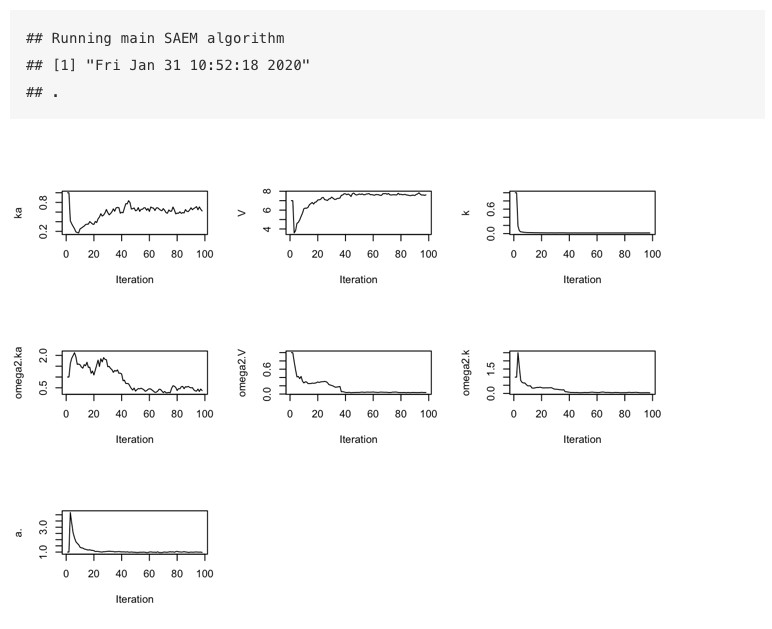
\includegraphics[width=1\linewidth]{figures/resultcase1} 

}

\end{figure}

\section{A categorical data model with regression
variables}\label{a-categorical-data-model-with-regression-variables}

\subsection{mlxR: simulate synthetic
data}\label{mlxr-simulate-synthetic-data}

\begin{Shaded}
\begin{Highlighting}[]
\KeywordTok{library}\NormalTok{(}\StringTok{"mlxR"}\NormalTok{)}
\NormalTok{catModel <-}\StringTok{ }\KeywordTok{inlineModel}\NormalTok{(}
\StringTok{"[LONGITUDINAL]}
\StringTok{input =  \{beta0,gamma0,delta0, dose\}}
\StringTok{dose = \{use=regressor\}}
\StringTok{EQUATION:}
\StringTok{lm0 = beta0+gamma0*t + delta0*dose}
\StringTok{D = exp(lm0)+1}
\StringTok{p0 = exp(lm0)/D}
\StringTok{p1 = 1/D}

\StringTok{DEFINITION:}
\StringTok{y = \{type=categorical, categories=\{0, 1\}, }
\StringTok{     P(y=0)=p0,}
\StringTok{     P(y=1)=p1\}}
\StringTok{[INDIVIDUAL]}
\StringTok{input=\{beta0_pop, o_beta0,}
\StringTok{      gamma0_pop, o_gamma0,}
\StringTok{      delta0_pop, o_delta0\}}
\StringTok{DEFINITION:}
\StringTok{beta0  =\{distribution=normal, prediction=beta0_pop,  sd=o_beta0\}}
\StringTok{gamma0  =\{distribution=normal, prediction=gamma0_pop,  sd=o_gamma0\}}
\StringTok{delta0  =\{distribution=normal, prediction=delta0_pop,  sd=o_delta0\} "}\NormalTok{)}

\NormalTok{nobs =}\StringTok{ }\DecValTok{15}
\NormalTok{tobs<-}\StringTok{ }\KeywordTok{seq}\NormalTok{(-}\DecValTok{20}\NormalTok{, }\DecValTok{50}\NormalTok{, }\DataTypeTok{by=}\NormalTok{nobs)}
\NormalTok{reg1 <-}\StringTok{ }\KeywordTok{list}\NormalTok{(}\DataTypeTok{name=}\StringTok{'dose'}\NormalTok{,}
            \DataTypeTok{time=}\NormalTok{tobs,}
            \DataTypeTok{value=}\DecValTok{10}\NormalTok{*(tobs>}\DecValTok{0}\NormalTok{))}

\NormalTok{reg2 <-}\StringTok{ }\KeywordTok{list}\NormalTok{(}\DataTypeTok{name=}\StringTok{'dose'}\NormalTok{,}
            \DataTypeTok{time=}\NormalTok{tobs,}
            \DataTypeTok{value=}\DecValTok{20}\NormalTok{*(tobs>}\DecValTok{0}\NormalTok{))}

\NormalTok{reg3 <-}\StringTok{ }\KeywordTok{list}\NormalTok{(}\DataTypeTok{name=}\StringTok{'dose'}\NormalTok{,}
            \DataTypeTok{time=}\NormalTok{tobs,}
            \DataTypeTok{value=}\DecValTok{30}\NormalTok{*(tobs>}\DecValTok{0}\NormalTok{))}

\NormalTok{out  <-}\StringTok{ }\KeywordTok{list}\NormalTok{(}\DataTypeTok{name=}\StringTok{'y'}\NormalTok{, }\DataTypeTok{time=}\NormalTok{tobs)}
\NormalTok{N  <-}\StringTok{ }\DecValTok{100}
\NormalTok{p <-}\StringTok{ }\KeywordTok{c}\NormalTok{(}\DataTypeTok{beta0_pop=}\NormalTok{-}\DecValTok{4}\NormalTok{, }\DataTypeTok{o_beta0=}\FloatTok{0.3}\NormalTok{, }
       \DataTypeTok{gamma0_pop=} \NormalTok{-}\FloatTok{0.5}\NormalTok{, }\DataTypeTok{o_gamma0=}\FloatTok{0.2}\NormalTok{,}
       \DataTypeTok{delta0_pop=}\DecValTok{1}\NormalTok{, }\DataTypeTok{o_delta0=}\FloatTok{0.2}\NormalTok{)}

\NormalTok{g1 <-}\StringTok{ }\KeywordTok{list}\NormalTok{(}\DataTypeTok{size=}\NormalTok{N,}\DataTypeTok{regressor =} \NormalTok{reg1)}
\NormalTok{g2 <-}\StringTok{ }\KeywordTok{list}\NormalTok{(}\DataTypeTok{size=}\NormalTok{N,}\DataTypeTok{regressor =} \NormalTok{reg2)}
\NormalTok{g3 <-}\StringTok{ }\KeywordTok{list}\NormalTok{(}\DataTypeTok{size=}\NormalTok{N,}\DataTypeTok{regressor =} \NormalTok{reg3)}
\NormalTok{g <-}\StringTok{ }\KeywordTok{list}\NormalTok{(g1,g2,g3)}
\NormalTok{res <-}\StringTok{ }\KeywordTok{simulx}\NormalTok{(}\DataTypeTok{model=}\NormalTok{catModel,}\DataTypeTok{output=}\NormalTok{out, }\DataTypeTok{group=}\NormalTok{g,}\DataTypeTok{parameter=}\NormalTok{p)}
\NormalTok{plot1 <-}\StringTok{ }\KeywordTok{catplotmlx}\NormalTok{(res$y)}
\end{Highlighting}
\end{Shaded}

\begin{figure}

{\centering 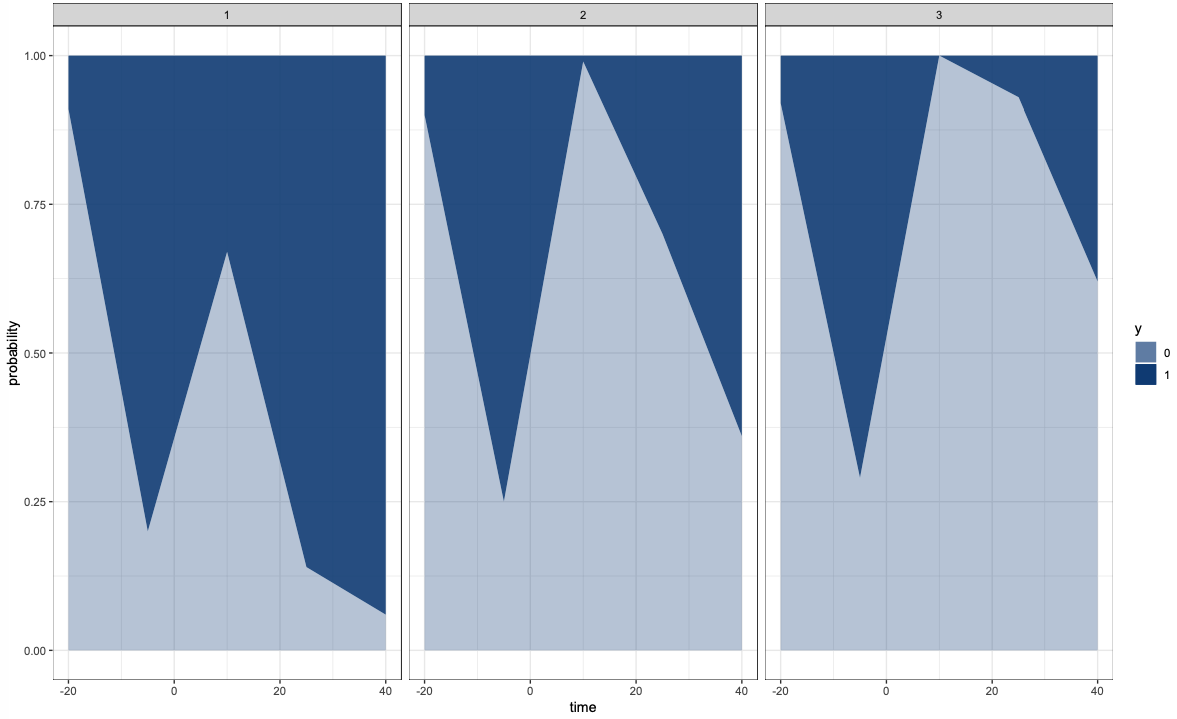
\includegraphics[width=1\linewidth]{figures/prob_cat} 

}

\end{figure}

\subsection{saemix: fit the noncontinuous data
model}\label{saemix-fit-the-noncontinuous-data-model}

\textbf{Create the saemix.data object}

\begin{Shaded}
\begin{Highlighting}[]
\NormalTok{saemix.data<-}\KeywordTok{saemixData}\NormalTok{(}\DataTypeTok{name.data=}\NormalTok{res,}\DataTypeTok{header=}\OtherTok{TRUE}\NormalTok{,}\DataTypeTok{sep=}\StringTok{" "}\NormalTok{,}
  \DataTypeTok{na=}\OtherTok{NA}\NormalTok{, }\DataTypeTok{name.group=}\KeywordTok{c}\NormalTok{(}\StringTok{"id"}\NormalTok{),}\DataTypeTok{name.predictors=}\KeywordTok{c}\NormalTok{(}\StringTok{"amount"}\NormalTok{,}\StringTok{"time"}\NormalTok{),}
  \DataTypeTok{name.response=}\KeywordTok{c}\NormalTok{(}\StringTok{"y1"}\NormalTok{), }\DataTypeTok{name.X=}\StringTok{"time"}\NormalTok{)}
\end{Highlighting}
\end{Shaded}

\textbf{Create the model}

\texttt{saemix} models are contained in a R function with one blocks:

\begin{Shaded}
\begin{Highlighting}[]
\NormalTok{cat.model<-function(psi,id,xidep) \{}
\NormalTok{level<-xidep[,}\DecValTok{1}\NormalTok{]}
\NormalTok{dose<-xidep[,}\DecValTok{2}\NormalTok{]}
\NormalTok{time<-xidep[,}\DecValTok{3}\NormalTok{]}
\NormalTok{th1 <-}\StringTok{ }\NormalTok{psi[id,}\DecValTok{1}\NormalTok{]}
\NormalTok{th2 <-}\StringTok{ }\NormalTok{psi[id,}\DecValTok{2}\NormalTok{]}
\NormalTok{delta0 <-}\StringTok{ }\NormalTok{psi[id,}\DecValTok{3}\NormalTok{]}
\NormalTok{lm0 <-}\StringTok{ }\NormalTok{th1+th2*time +}\StringTok{ }\NormalTok{delta0*dose}
\NormalTok{D <-}\StringTok{ }\KeywordTok{exp}\NormalTok{(lm0)+}\DecValTok{1}
\NormalTok{P0 <-}\StringTok{ }\KeywordTok{exp}\NormalTok{(lm0)/D}
\NormalTok{P1 <-}\StringTok{ }\DecValTok{1}\NormalTok{/D}

\NormalTok{P.obs =}\StringTok{ }\NormalTok{(level==}\DecValTok{0}\NormalTok{)*P0+(level==}\DecValTok{1}\NormalTok{)*P1}
\KeywordTok{return}\NormalTok{(P.obs) \}}

\NormalTok{saemix.model<-}\KeywordTok{saemixModel}\NormalTok{(}\DataTypeTok{model=}\NormalTok{cat.model,}\DataTypeTok{description=}\StringTok{"cat model"}\NormalTok{,}
  \DataTypeTok{type=}\StringTok{"likelihood"}\NormalTok{, }\DataTypeTok{psi0=}\KeywordTok{matrix}\NormalTok{(}\KeywordTok{c}\NormalTok{(}\DecValTok{2}\NormalTok{,}\DecValTok{1}\NormalTok{,}\DecValTok{2}\NormalTok{),}\DataTypeTok{ncol=}\DecValTok{3}\NormalTok{,}\DataTypeTok{byrow=}\OtherTok{TRUE}\NormalTok{,}
  \DataTypeTok{dimnames=}\KeywordTok{list}\NormalTok{(}\OtherTok{NULL}\NormalTok{,}\KeywordTok{c}\NormalTok{(}\StringTok{"th1"}\NormalTok{,}\StringTok{"th2"}\NormalTok{,}\StringTok{"th3"}\NormalTok{))),}\DataTypeTok{transform.par=}\KeywordTok{c}\NormalTok{(}\DecValTok{0}\NormalTok{,}\DecValTok{1}\NormalTok{,}\DecValTok{1}\NormalTok{),}
  \DataTypeTok{covariance.model=}\KeywordTok{matrix}\NormalTok{(}\KeywordTok{c}\NormalTok{(}\DecValTok{1}\NormalTok{,}\DecValTok{0}\NormalTok{,}\DecValTok{0}\NormalTok{,}\DecValTok{0}\NormalTok{,}\DecValTok{1}\NormalTok{,}\DecValTok{0}\NormalTok{,}\DecValTok{0}\NormalTok{,}\DecValTok{0}\NormalTok{,}\DecValTok{1}\NormalTok{),}\DataTypeTok{ncol=}\DecValTok{3}\NormalTok{,}\DataTypeTok{byrow=}\OtherTok{TRUE}\NormalTok{),}
  \DataTypeTok{omega.init=}\KeywordTok{matrix}\NormalTok{(}\KeywordTok{c}\NormalTok{(}\DecValTok{2}\NormalTok{,}\DecValTok{0}\NormalTok{,}\DecValTok{0}\NormalTok{,}\DecValTok{0}\NormalTok{,}\DecValTok{1}\NormalTok{,}\DecValTok{0}\NormalTok{,}\DecValTok{0}\NormalTok{,}\DecValTok{0}\NormalTok{,}\DecValTok{1}\NormalTok{),}\DataTypeTok{ncol=}\DecValTok{3}\NormalTok{,}\DataTypeTok{byrow=}\OtherTok{TRUE}\NormalTok{),}
  \DataTypeTok{error.model=}\StringTok{"constant"}\NormalTok{)}
\end{Highlighting}
\end{Shaded}

\textbf{Run the SAEM algorithm}

\begin{Shaded}
\begin{Highlighting}[]
\NormalTok{K1 =}\StringTok{ }\DecValTok{500}
\NormalTok{K2 =}\StringTok{ }\DecValTok{100}

\NormalTok{options<-}\KeywordTok{list}\NormalTok{(}\DataTypeTok{seed=}\DecValTok{39546}\NormalTok{,}\DataTypeTok{map=}\NormalTok{F,}\DataTypeTok{fim=}\NormalTok{F,}\DataTypeTok{ll.is=}\NormalTok{F,}
  \DataTypeTok{nbiter.mcmc =} \KeywordTok{c}\NormalTok{(}\DecValTok{2}\NormalTok{,}\DecValTok{2}\NormalTok{,}\DecValTok{2}\NormalTok{), }\DataTypeTok{nbiter.saemix =} \KeywordTok{c}\NormalTok{(K1,K2),}\DataTypeTok{nbiter.sa=}\DecValTok{0}\NormalTok{,}
  \DataTypeTok{displayProgress=}\OtherTok{TRUE}\NormalTok{,}\DataTypeTok{save.graphs=}\OtherTok{FALSE}\NormalTok{,}\DataTypeTok{nbiter.burn =}\DecValTok{0}\NormalTok{)}
\NormalTok{saemix.fit<-}\KeywordTok{saemix}\NormalTok{(saemix.model,saemix.data,options)}
\end{Highlighting}
\end{Shaded}

\begin{figure}

{\centering 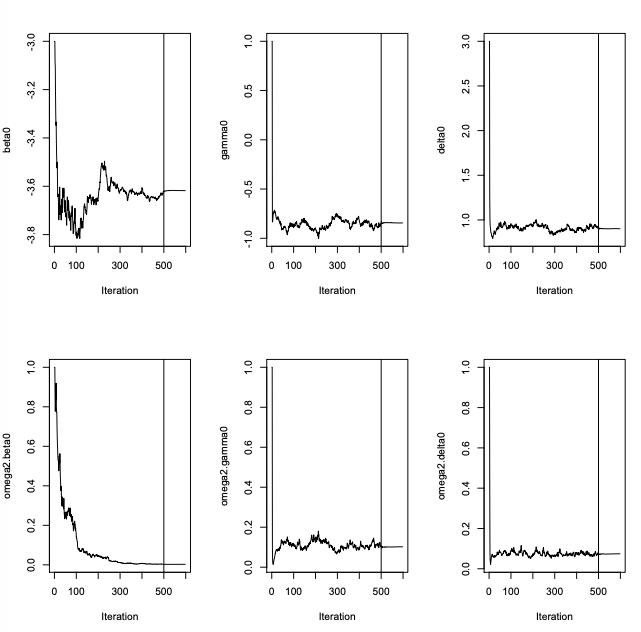
\includegraphics[width=1\linewidth]{figures/param_cat} 

}

\end{figure}

\section{A repeated time-to-event data
model}\label{a-repeated-time-to-event-data-model}

\textbf{Read the Data}

\begin{Shaded}
\begin{Highlighting}[]
\KeywordTok{data}\NormalTok{(tte.saemix)}
\NormalTok{saemix.data<-}\KeywordTok{saemixData}\NormalTok{(}\DataTypeTok{name.data=}\NormalTok{tte.saemix,}\DataTypeTok{header=}\OtherTok{TRUE}\NormalTok{,}
  \DataTypeTok{sep=}\StringTok{" "}\NormalTok{,}\DataTypeTok{na=}\OtherTok{NA}\NormalTok{, }\DataTypeTok{name.group=}\KeywordTok{c}\NormalTok{(}\StringTok{"id"}\NormalTok{),}
  \DataTypeTok{name.response=}\KeywordTok{c}\NormalTok{(}\StringTok{"y"}\NormalTok{),}\DataTypeTok{name.predictors=}\KeywordTok{c}\NormalTok{(}\StringTok{"time"}\NormalTok{,}\StringTok{"y"}\NormalTok{),}
  \DataTypeTok{name.X=}\KeywordTok{c}\NormalTok{(}\StringTok{"time"}\NormalTok{))}
\end{Highlighting}
\end{Shaded}

\textbf{Create the Model}

\texttt{saemix} models are contained in a R function with one blocks:

\begin{Shaded}
\begin{Highlighting}[]
\NormalTok{timetoevent.model<-function(psi,id,xidep) \{}
    \NormalTok{T<-xidep[,}\DecValTok{1}\NormalTok{]}
    \NormalTok{N <-}\StringTok{ }\KeywordTok{nrow}\NormalTok{(psi)}
    \NormalTok{Nj <-}\StringTok{ }\KeywordTok{length}\NormalTok{(T)}
    \NormalTok{censoringtime =}\StringTok{ }\DecValTok{20}
    \NormalTok{lambda <-}\StringTok{ }\NormalTok{psi[id,}\DecValTok{1}\NormalTok{]}
    \NormalTok{beta <-}\StringTok{ }\NormalTok{psi[id,}\DecValTok{2}\NormalTok{]}
    \NormalTok{init <-}\StringTok{ }\KeywordTok{which}\NormalTok{(T==}\StringTok{ }\DecValTok{0}\NormalTok{)}
    \NormalTok{cens <-}\StringTok{ }\KeywordTok{which}\NormalTok{(T==}\StringTok{ }\NormalTok{censoringtime)}
    \NormalTok{ind <-}\StringTok{ }\KeywordTok{setdiff}\NormalTok{(}\DecValTok{1}\NormalTok{:Nj, }\KeywordTok{append}\NormalTok{(init,cens))}
    \NormalTok{hazard <-}\StringTok{ }\NormalTok{(beta/lambda)*(T/lambda)^(beta}\DecValTok{-1}\NormalTok{)}
    \NormalTok{H <-}\StringTok{ }\NormalTok{(T/lambda)^beta}
    \NormalTok{logpdf <-}\StringTok{ }\KeywordTok{rep}\NormalTok{(}\DecValTok{0}\NormalTok{,Nj)}
    \NormalTok{logpdf[cens] <-}\StringTok{ }\NormalTok{-H[cens] +}\StringTok{ }\NormalTok{H[cens}\DecValTok{-1}\NormalTok{]}
    \NormalTok{logpdf[ind] <-}\StringTok{ }\NormalTok{-H[ind] +}\StringTok{ }\NormalTok{H[ind}\DecValTok{-1}\NormalTok{] +}\StringTok{ }\KeywordTok{log}\NormalTok{(hazard[ind])}
    \KeywordTok{return}\NormalTok{(logpdf) \}}


\NormalTok{saemix.model<-}\KeywordTok{saemixModel}\NormalTok{(}\DataTypeTok{model=}\NormalTok{timetoevent.model,}\DataTypeTok{description=}\StringTok{"time model"}\NormalTok{,}
  \DataTypeTok{type=}\StringTok{"likelihood"}\NormalTok{, }\DataTypeTok{psi0=}\KeywordTok{matrix}\NormalTok{(}\KeywordTok{c}\NormalTok{(}\DecValTok{2}\NormalTok{,}\DecValTok{1}\NormalTok{),}\DataTypeTok{ncol=}\DecValTok{2}\NormalTok{,}\DataTypeTok{byrow=}\OtherTok{TRUE}\NormalTok{,}
  \DataTypeTok{dimnames=}\KeywordTok{list}\NormalTok{(}\OtherTok{NULL}\NormalTok{, }\KeywordTok{c}\NormalTok{(}\StringTok{"lambda"}\NormalTok{,}\StringTok{"beta"}\NormalTok{))), }\DataTypeTok{transform.par=}\KeywordTok{c}\NormalTok{(}\DecValTok{1}\NormalTok{,}\DecValTok{1}\NormalTok{),}
  \DataTypeTok{covariance.model=}\KeywordTok{matrix}\NormalTok{(}\KeywordTok{c}\NormalTok{(}\DecValTok{1}\NormalTok{,}\DecValTok{0}\NormalTok{,}\DecValTok{0}\NormalTok{,}\DecValTok{1}\NormalTok{),}\DataTypeTok{ncol=}\DecValTok{2}\NormalTok{, }\DataTypeTok{byrow=}\OtherTok{TRUE}\NormalTok{))}
\end{Highlighting}
\end{Shaded}

\textbf{Run the SAEM algorithm}

\begin{Shaded}
\begin{Highlighting}[]
\NormalTok{K1 =}\StringTok{ }\DecValTok{200}
\NormalTok{K2 =}\StringTok{ }\DecValTok{100}

\NormalTok{saemix.options<-}\KeywordTok{list}\NormalTok{(}\DataTypeTok{map=}\NormalTok{F,}\DataTypeTok{fim=}\NormalTok{F,}\DataTypeTok{ll.is=}\NormalTok{F, }\DataTypeTok{nb.chains =} \DecValTok{1}\NormalTok{, }
  \DataTypeTok{nbiter.saemix =} \KeywordTok{c}\NormalTok{(K1,K2),}\DataTypeTok{displayProgress=}\OtherTok{TRUE}\NormalTok{,}\DataTypeTok{save.graphs=}\OtherTok{FALSE}\NormalTok{)}
\NormalTok{saemix.fit<-}\KeywordTok{saemix}\NormalTok{(model,saemix.data,saemix.options)}
\end{Highlighting}
\end{Shaded}

\begin{figure}

{\centering 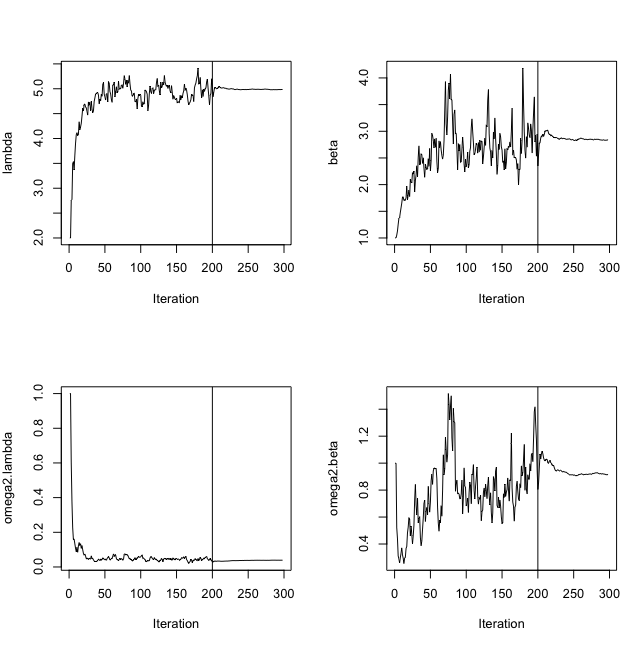
\includegraphics[width=1\linewidth]{figures/popparam_tte} 

}

\end{figure}

\chapter*{Contacts}\label{contacts}
\addcontentsline{toc}{chapter}{Contacts}

saemix is maintained by Emmanuelle Comets
(\href{mailto:emmanuelle.comets@inserm.fr}{\nolinkurl{emmanuelle.comets@inserm.fr}})
Inserm U738, Paris, France and CIC 0203, Rennes, France and Belhal
Karimi
(\href{mailto:belhal.karimi@polytechnique.edu}{\nolinkurl{belhal.karimi@polytechnique.edu}}).

Please address any questions, bug notice or suggestions.

\bibliography{book.bib,packages.bib}

\end{document}
